\chapter{Pipeline}

We consider a variant of problem \ref{prob:problem2} as follow:

\begin{problem}[Problem 3]:

Given a directed graph $G_P = (V_P, E_P)$ with triangle equality.

Find $K$ cycles that cover $V_P$.

\textbf{Objective:} Minimize the maximum of cycle length over all cycles.

\label{prob:problem3}
\end{problem}

The algorithm pipeline is as follow:

\begin{figure}[!h]
\centering
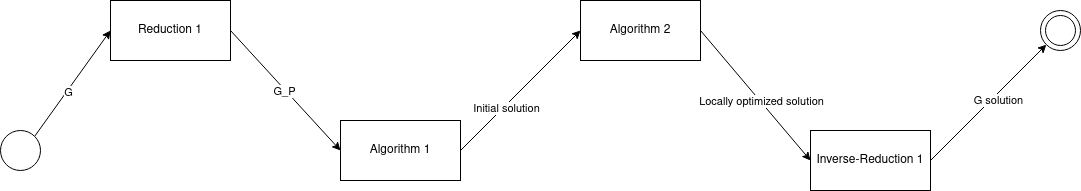
\includegraphics[width=1.2\textwidth]{assets/pipeline.png}
\caption{Pipeline}
\label{fig:pipeline}
\end{figure}

Reduction 1 converts a graph $G$ and a set of POIs $V_P$ to graph $G_P$. After that, Algorithm 1 and Algorithm 2 find a approximate-solution for problem \ref{prob:problem3}. Finally, Inverse-Reduction 1 converts the approximate-solution back to an approximate-solution for problem 1.